\documentclass[runningheads]{llncs}
\usepackage[T1]{fontenc}
\usepackage{graphicx}
\usepackage[table,xcdraw]{xcolor}
\usepackage{longtable}
\graphicspath{{Images}}

\begin{document}

\begin{titlepage}
    \centering
    {\bfseries\LARGE International University of Ecuador \par}
    \vspace{1cm}
    {\scshape\Large School of Mechatronics Engineering \par}
    \vspace{3cm}
    {\scshape\Huge Industrial Automation \\ Lab's report practice No. 1\par}
    \vspace{3cm}
    {\itshape\Large CADeSIMU Software and circuits implementation. \par}
    \vfill
    {\Large Authors: \par}
    {\Large Sebastian Osorio \par}
    {\Large Pablo Guacho \par}
    \vfill
    {\Large 2022-2023 \par}
\end{titlepage}
\newpage
\title{CADeSIMU software and circuits implementation\thanks{UIDE}}

\author{Sebastian Osorio\inst{1}\orcidID{0000-0003-0106-5482}
    \and
    Pablo Guacho\inst{1}\orcidID{0000-0003-0106-5482}
}

\authorrunning{S. Osorio, P. Guacho}

\institute{International University of Ecuador, Quito Av. Jorge Fernández and Av. Simón Bolívar 170201, Ecuador
    \email{uide@uide.edu.ec}
    \url{https://www.uide.edu.ec/} }

\maketitle


\section{CADeSIMU}
\begin{itemize}
    \item Using CADeSIMU software, implement the following circuit.Fig \ref{fig:CircuitToReplicate}
    \item Place the correct referencing, numbering, labeling, location in the circuit to be simulated. Explain how the circuit would work.
    \item Submit: Electric diagram implemented in CADeSIMU software in PDF format, CADeSIMU program in cad format.
    \item Make a summary table, indicating: nomenclature, symbols and a real image of each of the elements present in the scheme or diagram.
    \item Comment on the importance of labeling the terminals of the elements, contacts, coils, terminal blocks and connection cables in a control panel and electrical diagrams under the standard indicated in the previous literal.
\end{itemize}
\begin{figure}[!ht]
    \centering
    \caption{Circuit meant to be replicated.}\label{fig:CircuitToReplicate}
    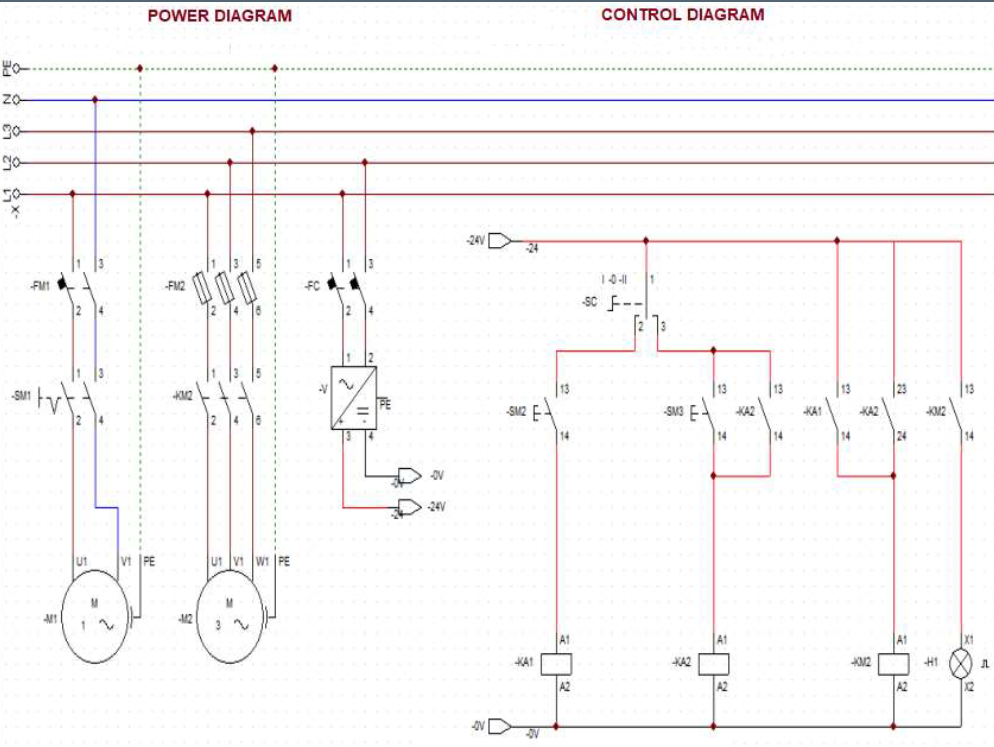
\includegraphics[width=\linewidth, height=7cm]{CircuitToReplicate.png}
\end{figure}

\newpage

\begin{figure}[!ht]
    \centering
    \caption{Circuit replicated and being simulated in CADeSIMU}\label{fig:CircuitSimulated}
    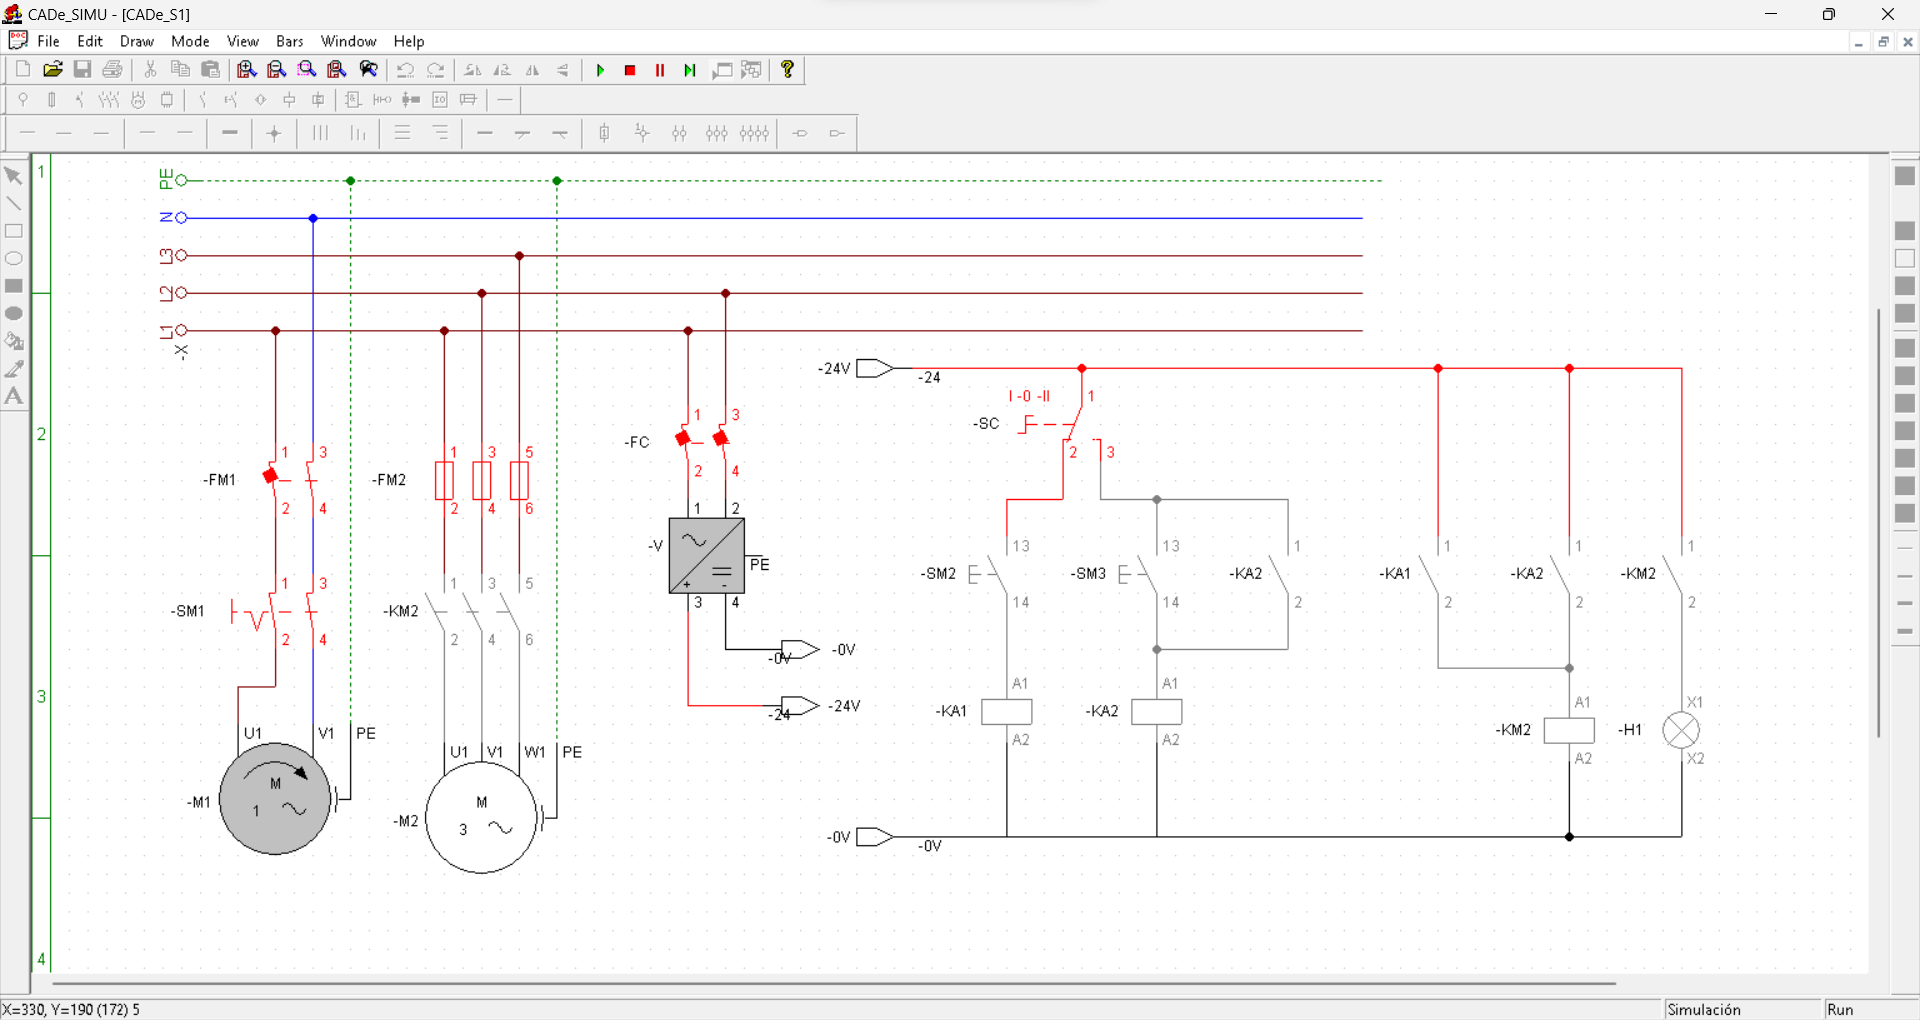
\includegraphics[width=\linewidth, height=7cm]{CircuitReplicated.png}
\end{figure}

\begin{figure}[!ht]
    \centering
    \caption{Final electrical plane with its references }\label{fig:CircuitPDF}
    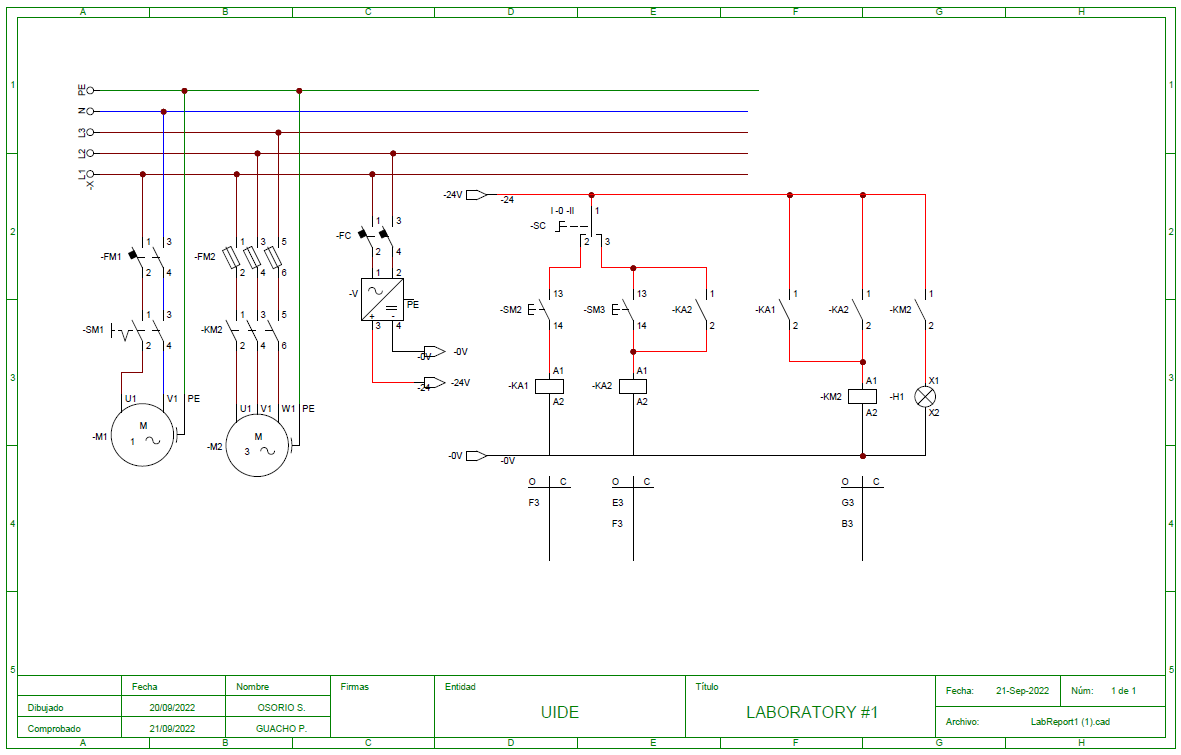
\includegraphics[width=\linewidth, height=7cm]{ReportLaboratoryNo1/Images/CircuitPDF.png}
\end{figure}

 \newpage
\subsection{Summary of the circuit components}

% Please add the following required packages to your document preamble:
% \usepackage[table,xcdraw]{xcolor}
% If you use beamer only pass "xcolor=table" option, i.e. \documentclass[xcolor=table]{beamer}
% \usepackage{longtable}
% Note: It may be necessary to compile the document several times to get a multi-page table to line up properly
\begin{longtable}{|
    >{\columncolor[HTML]{A6637E}}l |l|l|l|l|}
  \caption{Components summary.}
  \label{tab:CompSumary}                                                                                                                                                                                                              \\
  \hline
  \multicolumn{1}{|c|}{\cellcolor[HTML]{673147}{\color[HTML]{FFFFFF} No}}          &
  \multicolumn{1}{c|}{\cellcolor[HTML]{673147}{\color[HTML]{FFFFFF} Name}}         &
  \multicolumn{1}{c|}{\cellcolor[HTML]{673147}{\color[HTML]{FFFFFF} Nomenclature}} &
  \multicolumn{1}{c|}{\cellcolor[HTML]{673147}{\color[HTML]{FFFFFF} Symbol}}       &
  \multicolumn{1}{c|}{\cellcolor[HTML]{673147}{\color[HTML]{FFFFFF} Real Image}}                                                                                                                                                      \\ \hline
  \endfirsthead
  %
  \multicolumn{5}{c}%
  {{\bfseries Table \thetable\ continued from previous page}}                                                                                                                                                                         \\
  \hline
  \multicolumn{1}{|c|}{\cellcolor[HTML]{673147}{\color[HTML]{FFFFFF} No}}          &
  \multicolumn{1}{c|}{\cellcolor[HTML]{673147}{\color[HTML]{FFFFFF} Name}}         &
  \multicolumn{1}{c|}{\cellcolor[HTML]{673147}{\color[HTML]{FFFFFF} Nomenclature}} &
  \multicolumn{1}{c|}{\cellcolor[HTML]{673147}{\color[HTML]{FFFFFF} Symbol}}       &
  \multicolumn{1}{c|}{\cellcolor[HTML]{673147}{\color[HTML]{FFFFFF} Real Image}}                                                                                                                                                      \\ \hline
  \endhead
  %
  \cellcolor[HTML]{A6637E}{\color[HTML]{FFFFFF} 1}                                 & Automatic Switch  II & hola & \raisebox{-\totalheight}{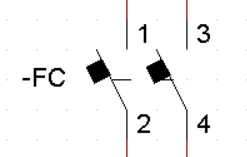
\includegraphics[width=3cm, height=3cm]{Device/AutomaticSwitchII.png}}  & AutomaticSwitchII  \\ \hline
  \cellcolor[HTML]{A6637E}{\color[HTML]{FFFFFF} 2}                                 & Automatic Switch IN  & hola & \raisebox{-\totalheight}{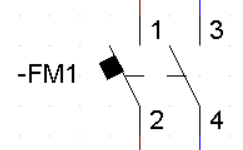
\includegraphics[width=3cm, height=3cm]{Device/AutomaticSwitchIN.png}}  & AutomaticSwitchIN  \\ \hline
  \cellcolor[HTML]{A6637E}{\color[HTML]{FFFFFF} 3}                                 & Coil contactor relay & - & \raisebox{-\totalheight}{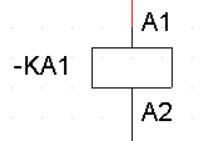
\includegraphics[width=3cm, height=3cm]{Device/CoilContactorRelay.png}} & CoilContactorRelay \\ \hline
  \cellcolor[HTML]{A6637E}{\color[HTML]{FFFFFF} 4}                                 & Contactor III        & - & \raisebox{-\totalheight}{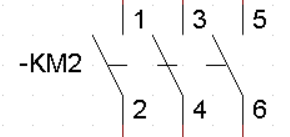
\includegraphics[width=3cm, height=3cm]{Device/ContactorIII.png}}       & ContactorIII       \\ \hline
  \cellcolor[HTML]{A6637E}{\color[HTML]{FFFFFF} 5}                                 & Double Interruptor   & - & \raisebox{-\totalheight}{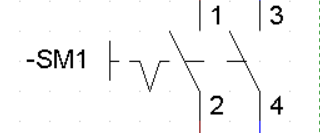
\includegraphics[width=3cm, height=3cm]{Device/doubleInterruptor.png}}  & doubleInterruptor  \\ \hline
  {\color[HTML]{FFFFFF} 6}                                                         & Fuse III             & - & \raisebox{-\totalheight}{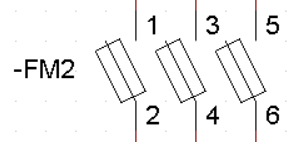
\includegraphics[width=3cm, height=3cm]{Device/FuseIII.png}}            & FuseIII            \\ \hline
  {\color[HTML]{FFFFFF} 7}                                                         & I O II Switch        & - & \raisebox{-\totalheight}{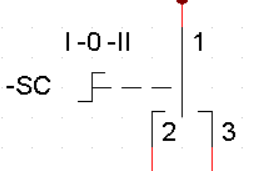
\includegraphics[width=3cm, height=3cm]{Device/I_0_II_Switch.png}}      & I\_0\_II\_Switch   \\ \hline
  {\color[HTML]{FFFFFF} 8}                                                         & Input Conector       & - & \raisebox{-\totalheight}{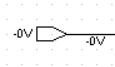
\includegraphics[width=3cm, height=3cm]{Device/inputConection.png}}     & inputConection     \\ \hline
  {\color[HTML]{FFFFFF} 9}                                                         & Mono-Phase Motor     & - & \raisebox{-\totalheight}{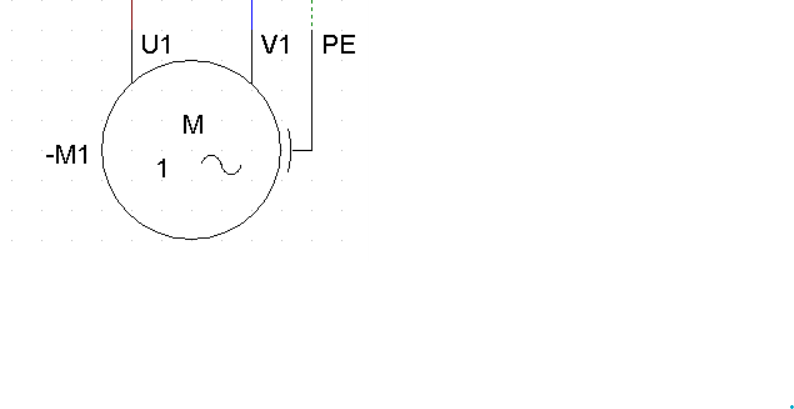
\includegraphics[width=3cm, height=3cm]{Device/monoPhaseMotor.png}}     & monoPhaseMotor     \\ \hline
  {\color[HTML]{FFFFFF} 10}                                                        & N-O Contact          & - & \raisebox{-\totalheight}{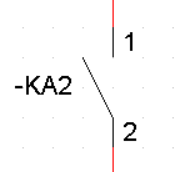
\includegraphics[width=3cm, height=3cm]{Device/NO_Contact.png}}         & NO\_Contact        \\ \hline
  {\color[HTML]{FFFFFF} 11}                                                        & Output Conector      & - & \raisebox{-\totalheight}{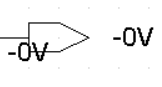
\includegraphics[width=3cm, height=3cm]{Device/outputConector.png}}     & outputConector     \\ \hline
  {\color[HTML]{FFFFFF} 12}                                                        & Pilot Signal         & - & \raisebox{-\totalheight}{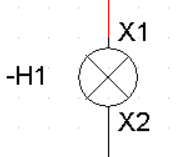
\includegraphics[width=3cm, height=3cm]{Device/PilotSignal.png}}        & PilotSignal        \\ \hline
  {\color[HTML]{FFFFFF} 13}                                                        & Power supply         & - & \raisebox{-\totalheight}{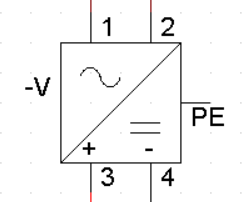
\includegraphics[width=3cm, height=3cm]{Device/powerSupply.png}}        & powerSupply        \\ \hline
  {\color[HTML]{FFFFFF} 14}                                                        & Push button          & - & \raisebox{-\totalheight}{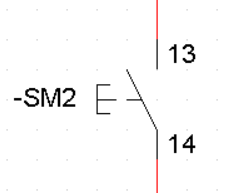
\includegraphics[width=3cm, height=3cm]{Device/pushbutton.png}}         & pushbutton         \\ \hline
  {\color[HTML]{FFFFFF} 15}                                                        & Three phase motor    & - & \raisebox{-\totalheight}{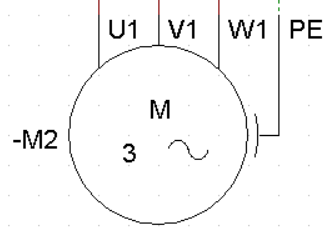
\includegraphics[width=3cm, height=3cm]{Device/ThreePhaseMotor.png}}    & ThreePhaseMotor    \\ \hline
\end{longtable}

\section{Conclusions and recommendations}
CADeSIMU is a very useful tool for electrical engineers, as it allows us to simulate any circuit and see if it works properly.
It has a very intuitive interface and is very easy to use, it also has a lot of components that can be used to simulate any circuit.
However, it is important it is important to understand and make use IEC 60617 standard in order to have a good labeling of the components like: 
contacts, coils, terminal blocks and connection cables.
They must be used correctly hence it helps to comprehend these diagrams and furthermore have an appropriate implementation of the circuit.
Moreover, it is important to have a good understanding of the components and how they work in order to be able to replicate the circuit. 
Also it is important to have a good understanding of the software and how to use it in order to be able to replicate the circuit.


% In case of adding a Bibliography just un-comment the following lines:
% \bibliographystyle{IEEEtrans}
% \bibliography{bibliography}
\end{document}